\documentclass[tikz,border=10pt]{standalone}
\usepackage{pgfplots}
\usetikzlibrary{intersections, calc}
\usepackage{ctex}
\begin{document}
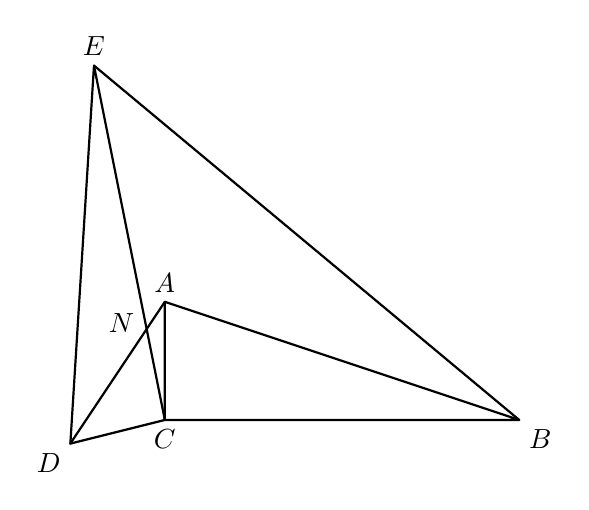
\begin{tikzpicture}[scale=1.5, >=stealth, line cap=round, line join=round]    
% 1. 定义核心顶点坐标 (基于视觉比例和常见几何模型设计)    
% 假设 C 为原点, CA 与 CB 垂直, CE 与 CD 垂直    
\coordinate (C) at (0, 0);    
\coordinate (A) at (0, 1);    
\coordinate (B) at (3, 0); 
\coordinate (D) at (-0.8, -0.2);    
\coordinate (E) at (-0.6, 3);
    % 2. 绘制主要线段    
% 绘制三角形 ABC    
\draw[thick] (A) -- (B) -- (C) -- cycle;
    % 绘制三角形 EDC    
\draw[thick] (E) -- (D) -- (C) -- cycle;
    % 绘制连接线 AD 和 EB    
\draw[thick, name path=lineAD] (A) -- (D);    
\draw[thick] (E) -- (B);
    % 3. 计算并标注交点 N (线段 AD 与 EC 的交点)    
\path[name path=lineEC] (E) -- (C);    
\fill [name intersections={of=lineAD and lineEC, by=N}]         
(N) circle (0pt); % 仅用于确定位置，不画实体点
    % 4. 标注字母文本    
\node[above] at (A) {$A$};    
\node[below right] at (B) {$B$};    
\node[below] at (C) {$C$};    
\node[below left] at (D) {$D$};    
\node[above] at (E) {$E$};    
\node[left, xshift=-1pt, yshift=2pt] at (N) {$N$};
\end{tikzpicture}
\end{document}